% $Header: /cvsroot/latex-beamer/latex-beamer/solutions/conference-talks/conference-ornate-20min.en.tex,v 1.6 2004/10/07 20:53:08 tantau Exp $

\documentclass{beamer}

% This file is a solution template for:

% - Talk at a conference/colloquium.
% - Talk length is about 20min.
% - Style is ornate.

\usepackage{amssymb}
\usepackage{amsmath}
\usepackage{amscd}
\newcommand{\abs}[1]{\left| #1 \right|}
\newcommand{\R}{\mathbb{R}}

% Copyright 2004 by Till Tantau <tantau@users.sourceforge.net>.
%
% In principle, this file can be redistributed and/or modified under
% the terms of the GNU Public License, version 2.
%
% However, this file is supposed to be a template to be modified
% for your own needs. For this reason, if you use this file as a
% template and not specifically distribute it as part of a another
% package/program, I grant the extra permission to freely copy and
% modify this file as you see fit and even to delete this copyright
% notice. 


\mode<presentation>
{
  \usetheme{CambridgeUS}
  % or ...

  \setbeamercovered{transparent}
  % or whatever (possibly just delete it)
}


\usepackage[english]{babel}
% or whatever

\usepackage{multicol, hyperref}

\usepackage[latin1]{inputenc}
% or whatever

\usepackage{times}
\usepackage[T1]{fontenc}
% Or whatever. Note that the encoding and the font should match. If T1
% does not look nice, try deleting the line with the fontenc.

\usepackage{graphicx}
\usepackage{caption}

\title
{Washington Experimental Mathematics Lab} % (optional, use only with long paper titles)

\subtitle
{Stability Spectrum for PDEs}

\date{Spring 2018}

\author{Faculty Mentor: Dr. Bernard Deconinck \\ Graduate Mentor: Jeremy Upsal \\ Team Members: Kush Gupta, Ryan Bushling}

% - Give the names in the same order as the appear in the paper.
% - Use the \inst{?} command only if the authors have different
%   affiliation.

\institute[University of Washington] % (optional, but mostly needed)
{
%  \inst{1}%
  Department of Mathematics\\
  University of Washington}
  %\and
  %\inst{2}%
  %Department of Theoretical Philosophy\\
  %University of Elsewhere}
% - Use the \inst command only if there are several affiliations.
% - Keep it simple, no one is interested in your street address.

%\date[CFP 2003] % (optional, should be abbreviation of conference name)
%{ REGS 2011 }
% - Either use conference name or its abbreviation.
% - Not really informative to the audience, more for people (including
%   yourself) who are reading the slides online

% This is only inserted into the PDF information catalog. Can be left
% out. 



% If you have a file called "university-logo-filename.xxx", where xxx
% is a graphic format that can be processed by latex or pdflatex,
% resp., then you can add a logo as follows:



% Delete this, if you do not want the table of contents to pop up at
% the beginning of each subsection:
%\AtBeginSubsection[]
%{
%  \begin{frame}<beamer>
%    \frametitle{Outline}
%    \tableofcontents[currentsection,currentsubsection]
%  \end{frame}
%}


% If you wish to uncover everything in a step-wise fashion, uncomment
% the following command: 

%\beamerdefaultoverlayspecification{<+->}


\begin{document}

\begin{frame}
  \titlepage
\end{frame}




% Structuring a talk is a difficult task and the following structure
% may not be suitable. Here are some rules that apply for this
% solution: 

% - Exactly two or three sections (other than the summary).
% - At *most* three subsections per section.
% - Talk about 30s to 2min per frame. So there should be between about
%   15 and 30 frames, all told.

% - A conference audience is likely to know very little of what you
%   are going to talk about. So *simplify*!
% - In a 20min talk, getting the main ideas across is hard
%   enough. Leave out details, even if it means being less precise than
%   you think necessary.
% - If you omit details that are vital to the proof/implementation,
%   just say so once. Everybody will be happy with that.



%\begin{frame}
 % \frametitle{Make Titles Informative.}

  %You can create overlays\dots
  %\begin{itemize}
  %\item using the \texttt{pause} command:
   % \begin{itemize}
    %\item
     % First item.
      %\pause
    %\item    
      %Second item.
    %\end{itemize}
 % \item
  %  using overlay specifications:
   % \begin{itemize}
    %\item<3->
     % First item.
    %\item<4->
     % Second item.
    %\end{itemize}
  %\item
   % using the general \texttt{uncover} command:
    %\begin{itemize}
     % \uncover<5->{\item
      %  First item.}
      %\uncover<6->{\item
       % Second item.}
    %\end{itemize}
  %\end{itemize}
%\end{frame}

% \section{Project Goals}

\begin{frame}{Stability Spectrum for PDEs}

\begin{description}

\item[Motivation] To determine the stability of periodic solutions to certain PDEs, including the focusing mKdV equation

\item[Problem] To determine the eigenvalues of a linear operator such that the associated eigenfunctions are bounded

\item[Methods] Taking advantage of the periodicity of the coefficients using Floquet theory and Fourier series

\end{description}

\end{frame}

\begin{frame}{Example}
  Let $\mathcal{L} = -\partial_{x}^2$ and consider the eigenvalue problem $$\mathcal{L}y = \lambda y, \qquad \lambda \in \mathbb{C},$$ or equivalently, $ y'' + \lambda y = 0$.
  \\
  \vspace{10mm}
  We say $\lambda \in \sigma(\mathcal{L})$ if the associated $y(x)$ is bounded for all $x\in \R$,  $\lim_{\abs{x}\to\infty}\abs{y(x)}<\infty$.
\end{frame}


\begin{frame}{Example (ct'd.)}

To find $\sigma(\mathcal{L})$, we solve the differential equation $ y'' + \lambda y = 0$. The general solution is \vspace*{-0.5cm}

\begin{align*}
 y &= c_1 \mathrm{e}^{\sqrt{-\lambda} x} + c_2 \mathrm{e}^{-\sqrt{-\lambda} x}. 
\end{align*}

In general, $\sqrt{-\lambda} \in \mathbb{C}$, so let $\sqrt{-\lambda} = \alpha + \mathrm{i} \beta$ for some $\alpha, \beta \in \mathbb{R}$.

\end{frame}


\begin{frame}{Example (ct'd.)}

Letting $\sqrt{-\lambda} = \alpha + \mathrm{i} \beta$, rewrite $y = c_1 \mathrm{e}^{\sqrt{-\lambda} x} + c_2 \mathrm{e}^{-\sqrt{-\lambda} x}$ as
\begin{align*}
y &= c_1 \mathrm{e}^{(\alpha + \mathrm{i} \beta) x} + c_2 \mathrm{e}^{-(\alpha + \mathrm{i} \beta) x} \\
    &= c_1 \mathrm{e}^{\alpha x} \mathrm{e}^{\mathrm{i} \beta x} + c_2 \mathrm{e}^{-\alpha x} \mathrm{e}^{-\mathrm{i} \beta x} \\
    &= c_1 \mathrm{e}^{\alpha x} [\cos(\beta x) + \mathrm{i} \sin(\beta x)] + c_2 \mathrm{e}^{-\alpha x} [\cos(\beta x) - \mathrm{i} \sin(\beta x)]
\end{align*}

We require that the solution $\lim_{\abs{x}\to\infty}\abs{y(x)}<\infty.$ Therefore, $\alpha =0$.

\end{frame}

\begin{frame}{Example (ct'd.)}

With $\alpha = 0$,
\begin{align*}
y &= c_1 [\cos(\beta x) + \mathrm{i} \sin(\beta x)] + c_2  [\cos(\beta x) - \mathrm{i} \sin(\beta x)] \\
&= A\cos(\beta x) + \mathrm{i}B \sin(\beta x)
\end{align*}
is bounded for any $\beta \in \mathbb{R}$. $\sqrt{-\lambda} = \mathrm{i} \beta$ only if $\lambda \geq 0$. 

So $\sigma(-\partial_{xx}) = [0,\infty)$. 

\end{frame}

% \section{Reporting}

\begin{frame}{Numerically computed spectrum}
\begin{figure}
\begin{center}
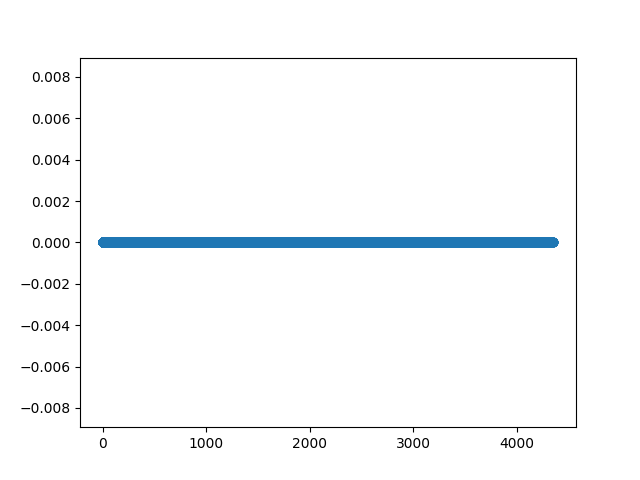
\includegraphics[scale=0.4]{dxxSpectrum.png}
\end{center}
\caption{Spectrum of the operator $\mathcal{L} = -\partial_{x}^2$.}
\end{figure}

\end{frame}

%\begin{frame}{Pictures}
%
%\begin{figure}
%\begin{center}
%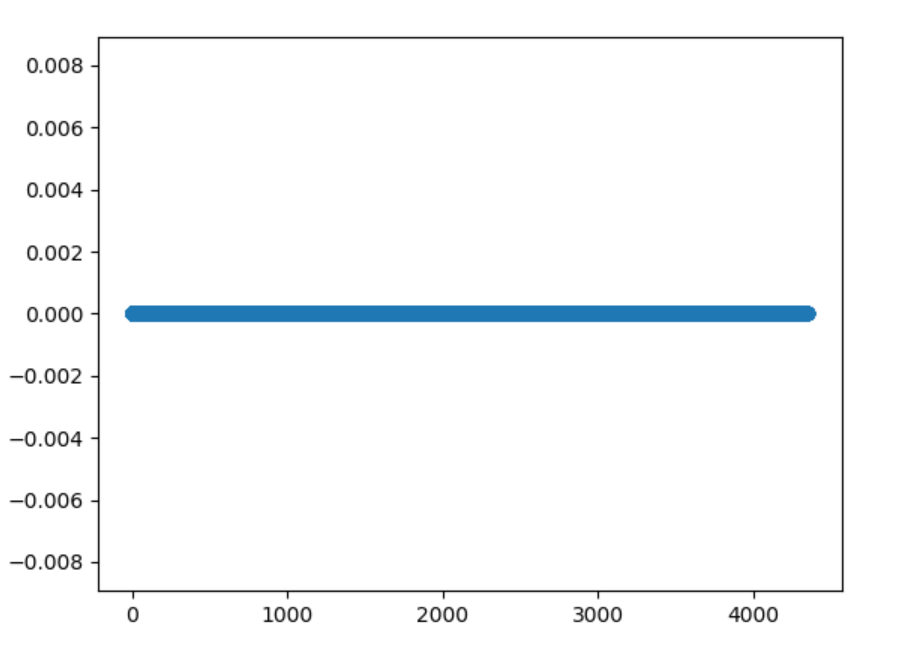
\includegraphics[scale=0.5]{FFHM_Spectrum_Example03.PNG}
%\end{center}
%\caption{Spectrum of the operator $\mathcal{L} = -\partial_{x}^2 + 2q\cos(2x)$ for $q=2$.}
%\end{figure}

%\end{frame}

\begin{frame}{Pictures}

\begin{figure}
\centering\captionsetup{width =\dimexpr\textwidth-2cm, format=hang}
 \begin{center}
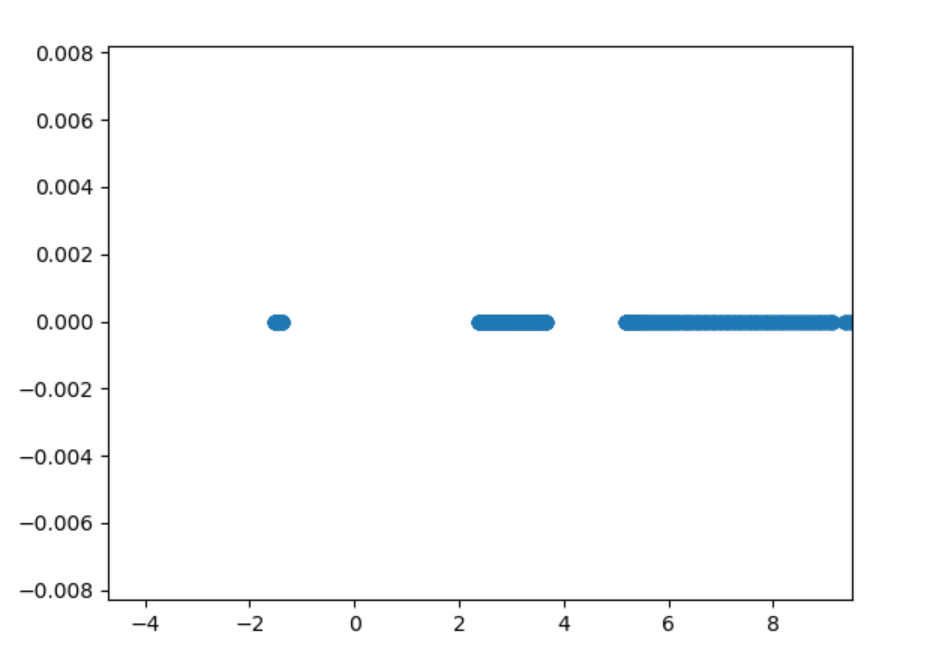
\includegraphics[scale=0.35]{FIXED_Spectrum_Plot_Example03.PNG}
 \end{center}
 \captionsetup{format=hang}
\caption{Spectrum of the operator $\mathcal{L} = -\partial_{x}^2 + 2q\cos(2x)$ \\ for $q=2$ from 0 to 10.}

\end{figure}

\end{frame}

% \begin{frame}{Progress}


% \begin{description}

% \item[What's worked] 

% \item[What hasn't] 

% \end{description}

% \end{frame}

% \section{What's next}

\begin{frame}{Future goals}

\begin{description}

\item[Next steps] Determining the spectrum of 
\begin{align*}
\mathcal{L} = -\partial_{y}^3 + (c - 6U^2)\partial_y + 12 U U_y,
\end{align*}
which is used in determining the stability of the solution $u(x,t) = U(y) = U(x-ct)$ of the focusing mKdV equation:
\begin{align*}
u_t + 6u^2 u_x + u_{xxx} = 0.
\end{align*}

\item[Challenges] Understanding elliptic functions and generalizing our code.

\end{description}

\end{frame}



\end{document}


